\documentclass[]{emse-exo}

\annee{}
\module{Master MISPA}
\matiere{}
\type{Tutorial}
\usepackage{graphics}
\graphicspath{{../../../book/media/}}

% ---------------------------------------
\usepackage{emselip}

% --------------------------------------
% TIKZ and diagrams
\usepackage{pgf,tikz}
\usetikzlibrary{arrows,shapes,matrix,positioning}
% styles de block pour diagrammes
\tikzset{decision/.style={diamond, draw, fill=blue!20, text width=1.5cm, text badly centered, inner sep=0pt, minimum width=3.5cm}}
\tikzset{block/.style={rectangle, draw, fill=blue!20, text width=3cm, text badly centered, rounded corners,
minimum width=3cm}}
\tikzset{dligne/.style={draw, latex-latex}}
\tikzset{ligne/.style={draw, -latex}}

\tikzset{title/.style={font=\fontsize{6}{6}\color{black!50}\ttfamily}}
\tikzset{typetag/.style={rectangle, draw=black!50, font=\scriptsize\ttfamily, anchor=west}}



% package pour l'insertion d'un espace intelligent
\usepackage{xspace}
% tilde in math mode
\renewcommand{\t}[1]{\ensuremath{\mathop{\tilde{#1}}\nolimits}}
\newcommand{\h}[1]{\ensuremath{\mathop{\hat{#1}}\nolimits}}
\newcommand{\lab}{$L^*a^*b^*$\xspace}
\newcommand{\argyb}{$(a,rg,yb)$\xspace}
\newcommand{\targyb}{$(\tilde{a},\tilde{rg},\tilde{yb})$\xspace} % tilde
\newcommand{\cargyb}{$(\h{a},\h{rg},\h{yb})$\xspace} % espace chapeau

\begin{document}
\def\QRCODE{TB_image_TUT.IMG.image_registration_pythonqrcode.png}
\def\QRPAGE{http://www.iptutorials.science/tree/master/TB_image/TUT.IMG.image_registration/python}
\pcorrectionsection{Python correction}

\begin{python}
from scipy import misc
import matplotlib.pyplot as plt
import numpy as np
import cv2
from scipy.spatial import cKDTree
\end{python}


\subsection{Transformation estimation based on corresponding points}
\subsubsection{Image visualization}
The following code is used to display the images (see Fig.\ref{fig:registration:python:initial}).

\begin{python}# Read images and display
A=imageio.imread("brain1.bmp")
B=imageio.imread("brain2.bmp")
plt.imshow(A,cmap='gray');
plt.show();
plt.imshow(B,cmap='gray');
plt.show();

# define control points
A_points = np.array([[136, 100], [127, 153], [96, 156], [87, 99]]);
B_points = np.array([[144, 99], [109, 140], [79, 128], [100, 74]]);
\end{python}

\begin{figure}[htbp]
\centering\caption{Initial images.}%
 \subfloat[Moving image.]{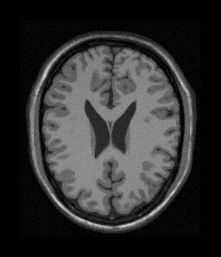
\includegraphics[width=.3\linewidth]{brain1.png}}\hfill
 \subfloat[Source image.]{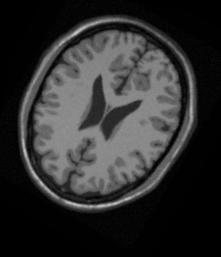
\includegraphics[width=.3\linewidth]{brain2.png}}\hfill
 \subfloat[Superimposition.]{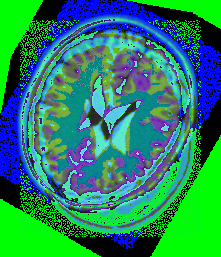
\includegraphics[width=.3\linewidth]{superimpose.png}}%
 \label{fig:registration:python:initial}%
\end{figure}

If you want to display and save the fusion of both images, you can use this function:
\begin{python}
def superimpose(G1, G2, filename=None):
    """
    superimpose 2 images, supposing they are grayscale images and of same shape
    """
    r,c=G1.shape;
    S = np.zeros((r,c,3));
    S[:,:,0] = np.maximum(G1-G2, 0)+G1;
    S[:,:,1] = np.maximum(G2-G1, 0)+G2;
    S[:,:,2] = (G1+G2) / 2;
    S = 255 * S / np.max(S);
    S = S.astype('uint8');
    plt.imshow(S);
    plt.show()    
    if filename!=None:
        cv2.imwrite(filename, S);
    return S
\end{python}


\subsubsection{Manual selection of corresponding points}
With openCV, there is not built-in function to make a manual selection of pairs of control points. The following code uses a global variable I in order to manage the display of the points, which are finally stored into the pts variable. First, the callback function \pinline{on_mouse} is defined to handle mouse event. 

\begin{python}
pts = [];
def on_mouse(event, x, y, flags, param):
    """
    callback method for detecting click on image
    It draws a circle on the global variable image I
    """
    global pts, I;
    if event == cv2.EVENT_LBUTTONUP:
        pts.append((x, y));
        cv2.circle(I,(x,y), 2, (0,0,255), -1)
\end{python}
The function \pinline{cpselect} allows the selection of multiple points.
\begin{python}
def cpselect():
    """
    method for manually selecting the control points
    It waits until 'q' key is pressed.
    """
    cv2.namedWindow("image")
    cv2.setMouseCallback("image", on_mouse)
    print("press 'q' when finished")
    # keep looping until the 'q' key is pressed
    while True:
    	# display the image and wait for a keypress
    	cv2.imshow("image", I)
    	key = cv2.waitKey(1) & 0xFF
    
    	# if the 'c' key is pressed, break from the loop
    	if key == ord("q"):
    		break

    # close all open windows
    cv2.destroyAllWindows()
    return pts;
\end{python}

\subsubsection{Transformation estimation}
The rigid transformation is estimated from the corresponding points by the following function:
\begin{python}
def rigid_registration(data1, data2):
    """
    Rigid transformation estimation between n pairs of points
    This function returns a rotation R and a translation t
    data1 : array of size nx2
    data2 : array of size nx2
    returns transformation matrix T of size 2x3
    """
    data1 = np.array(data1);
    data2 = np.array(data2);

    # computes barycenters, and recenters the points
    m1 = np.mean(data1,0);
    m2 = np.mean(data2,0);
    data1_inv_shifted = data1-m1;
    data2_inv_shifted = data2-m2;

    # Evaluates SVD
    K = np.matmul(np.transpose(data2_inv_shifted), data1_inv_shifted);
    U,S,V = np.linalg.svd(K);

    # Computes Rotation
    S = np.eye(2);
    S[1,1] = np.linalg.det(U)*np.linalg.det(V);
    R = np.matmul(U,S);
    R = np.matmul(R, np.transpose(V));

    # Computes Translation
    t = m2-np.matmul(R, m1);
    
    T = np.zeros((2,3));
    T[0:2,0:2] = R;
    T[0:2,2] = t;
    return T;
\end{python}
\smallskip
Then, you can apply this function to the manually selected points.
\smallskip
\begin{python}
# 1st case, rigid registration, with pairs of points in the correct order
T = rigid_registration(A_points, B_points);

# Apply transformation on control points and display the results
data_dest = applyTransform(A_points, T);
I = B.copy();
for pb,pa in zip(data_dest, B_points):
    cv2.circle(I,totuple(pa), 1, (255,0,0), -1)    
    cv2.circle(I,totuple(pb), 1, (0,0,255), -1)   
plt.imshow(I);
plt.show();
# Apply transformation on image
rows, cols= B.shape;
dst = cv2.warpAffine(A,T, (cols, rows));
plt.imshow(dst);
superimpose(dst, B, "rigid_manual.png");
\end{python}

\begin{figure}[htbp]
\centering\caption{Result of the registration for the manually selected control points.}%
 \subfloat[Without registration.]{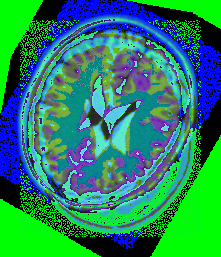
\includegraphics[width=.35\linewidth]{superimpose.png}}\hspace*{1.5cm}
 \subfloat[With registration.]{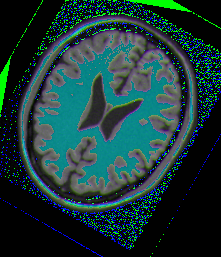
\includegraphics[width=.35\linewidth]{rigid_manual.png}}%
 \label{fig:registration:python:reg}%
\end{figure}

The result is good, because the manual selection of the points is good (the points are given in the correct order for both images).


\subsection{ICP registration}

\subsubsection{Random permutation of points}
The following code randomly shuffles the points of the first vector. The result is of course a wrongly registered image, see Fig.\ref{fig:registration:python:random}. 

\begin{python}
# random permutation of the points
p = np.random.permutation(np.arange(4));
A_points = A_points[p];
T = rigid_registration(A_points, B_points);
\end{python}

\begin{figure}[htbp]
\centering\caption{Result of the registration for when the control points are not found in the same order.}%
 \subfloat[Matching pairs of points.]{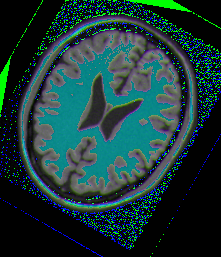
\includegraphics[width=.35\linewidth]{rigid_manual.png}}\hspace*{1.5cm}
 \subfloat[Permulation of the points.]{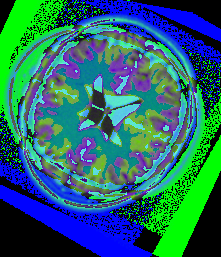
\includegraphics[width=.35\linewidth]{rigid_random_manual.png}}%
 \label{fig:registration:python:random}%
\end{figure}


\subsubsection{ICP}
The previous operations simulates a general non-manual selection of the control points: there is not reason to finding the points by matching pairs. Thus, a reordering is necessary. This propositions implies that the number of points is exactly the same in order to perform the registration process, and that these are matching points (every point has a matching point in the other image). The ICP method (see code for \pinline{icp_transform}) reorders the points via a nearest neighbor rule.

\begin{python}
def icp_transform(dataA, dataB):
    """
    Find a transform between A and B points
    with an ICP (Iterative Closest Point) method.
    dataA and dataB are of size nx2, with the same number of points n 
    returns the transformation matrix of shape 2x3
    """
    data2A = dataA.copy();
    data2B = np.zeros(data2A.shape);  
    T = np.zeros((2,3));
    T[0:2,0:2] = np.eye(2);
    T[0:2,2] = 0;
    
    nb_loops=5;
    tree = cKDTree( dataB );
    
    for loop in range(nb_loops):
        # search for closest points and reorganise array of points accordingly
        d, inds = tree.query( data2A);
        
        data2B = dataB[inds,:];
        # find rigid registration with reordered points
        t_loop = rigid_registration(data2A, data2B);
        
        T = composeTransform(t_loop, T);
        # evaluates transform on control points, to make the iteration
        data2A = applyTransform(dataA, T);
        
    return T;
\end{python}


\begin{figure}[htbp]
\centering\caption{Result of the registration for when the control points are not found in the same order. The ICP algorithm reorders the points and gives a good result.}%
 \subfloat[Random shuffle of points and direct rigid transformation estimation.]{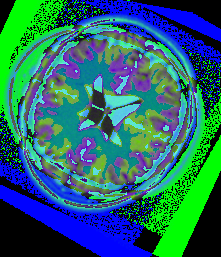
\includegraphics[width=.35\linewidth]{rigid_random_manual.png}}\hspace*{1.5cm}
 \subfloat[ICP registration on the same points.]{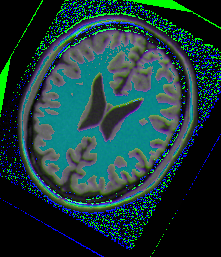
\includegraphics[width=.35\linewidth]{random_icp_manual.png}}%
 \label{fig:registration:python:icp}%
\end{figure}

\subsubsection{Automatic extraction of corner points}
Generally, the points are automatically detected, and thus, there is no warranty that they are found in the same order, nor that each pair of point correspond to matching points (some points --called outliers-- need to be eliminated to compute the correct transformation). In this tutorial, we do not address the problem of outliers. Please notice that with these parameters and images, by chance, the same points are detected in the correct order.

\begin{python}
# Automatic extraction of corner points
# Harris corners detection or Shi and Tomasi
# this method do not ensure the correct order in the points (A_points and 
# B_points)
nb_points = 4; # number of points to detect
corners = cv2.goodFeaturesToTrack(A,nb_points,0.01,10, blockSize=3, useHarrisDetector=False)
corners = np.int0(corners)
a, b, c = corners.shape;
A_points = np.reshape(corners, (a,c));

corners = cv2.goodFeaturesToTrack(B,nb_points,0.01,10, blockSize=3, useHarrisDetector=False)
corners = np.int0(corners)
a, b, c = corners.shape;
B_points = np.reshape(corners, (a,c));
\end{python}



The Fig.\ref{fig:registration:python:harris} displays the results with the automatic detection of corners (in this case, the method from Shi and Tomasi). Notice that by chance, the points in both images match. In other cases, one would have to remove outliers.

\begin{figure}[htbp]
\centering\caption{Shi and Tomasi corners detection. By chance, the points correspond and the ICP method gives a correct result.}%
 \subfloat[]{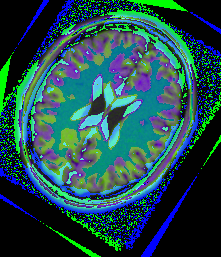
\includegraphics[width=.4\linewidth]{rigid_shitomasi.png}}\hfill
 \subfloat[]{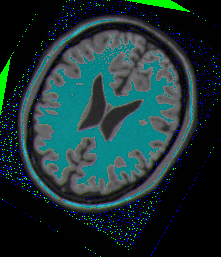
\includegraphics[width=.4\linewidth]{icp_shitomasi.png}}%
 \label{fig:registration:python:harris}%
\end{figure}



 \bibliographystyle{plain}
 \bibliography{colip.bib}
\end{document}
